\documentclass[10pt,a4paper]{article}
\usepackage{graphicx}
\usepackage{datetime}
\usepackage{color}
\usepackage[ latin1 ]{ inputenc }
\usepackage{wrapfig}
\usepackage{hyperref}
\usepackage{color}
\usepackage{ mathpazo }
\usepackage[ T1 ]{ fontenc }
\usepackage[font+=small]{sub caption}
\usepackage[font=small,labelfont=bf]{caption}
% load some useful math symbols / fonts
%\usepackage{ latexsym , amsfonts , amsmath , amssymb }
\usepackage[top =1 in ,bottom =1in ,left =1 in ,right =1 in ]{geometry}
\usepackage{natbib}
% control some spacings
%
% spacing after a paragraph
\setlength{\parskip }{.15 cm }
% indentation at the top of a new paragraph
\setlength{\parindent }{0.0 cm }
\begin{document}
\begin{center}
	\section* {Parameter Space Results for LMC SNRs}
\end{center}
Next few pages show parameter spaces for the 4 parameters in our model :-
\begin{itemize}
\item Fraction of Ia/CCs - $f$
\item SN Rate (Ia + CC) - $R$
\item Scale Height of HI disk - $z_0$
\item Schmidt-Kennicutt Law Index - $\alpha$\\
\end{itemize}
Parameters are constrained using 3 sets of observations :-
\begin{itemize}
\item Luminosity Distribution
\item Diameter Distribution
\item Ambient (Column) Density Distribution\\
\end{itemize}
The plots show confidence intervals calculated using log-likelihood described in my previous write-up (See Appendix A) for all SNRs brighter than $L_{cut}$.\\\\\\
Figs. 1-3 show the parameter space by luminosity, diameter and density comparison for $L_{cut} = 2 \times 10^{23}$ ergs/s/Hz.\\\\\\
Figs. 4-6 show the same for $L_{cut} = 9 \times 10^{22}$ ergs/s/Hz\\\\\\
Keep in mind the contours are \textbf{interpolated}: Due to runtime issues, I only sample ($5 \times 5$) data points for each parameter pair, marginalize over the nuisance parameters and calculate the log-likelihood. The contours are then constructed by interpolating between these 25 log-likelihood values.\\\\
\newpage
\section* {Luminosity Comparison ($L_{cut} = 2 \times 10^{23}\ ergs/s/Hz$)}
\begin{figure}[h!]
%\vspace{-10cm}
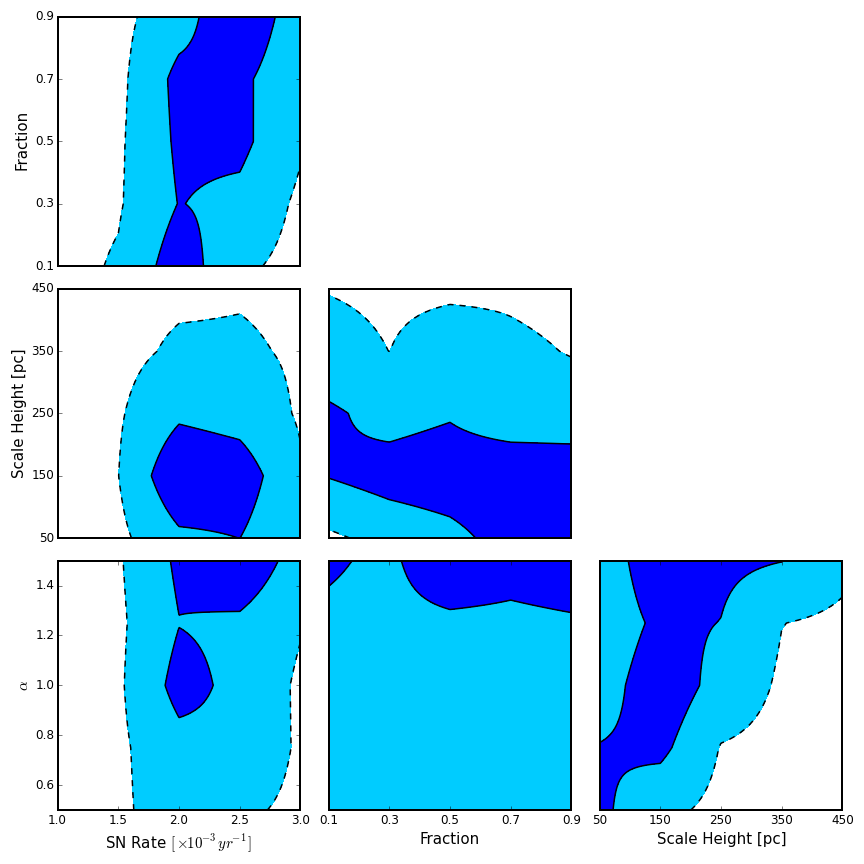
\includegraphics[width=15cm]{TrianglePlot_Lums.png}
\caption{Parameter Space constructed from comparing observed vs. model luminosity distribution for all Supernova brighter than $L_{cut}$. 65$\%$ region is shown in blue with solid border. 95$\%$ region is shown in cyan with dashed border.}
\end{figure}
\newpage
\section* {Diameter Comparison ($L_{cut} = 2 \times 10^{23}\ ergs/s/Hz$)}
\begin{figure}[h!]
%\vspace{-10cm}
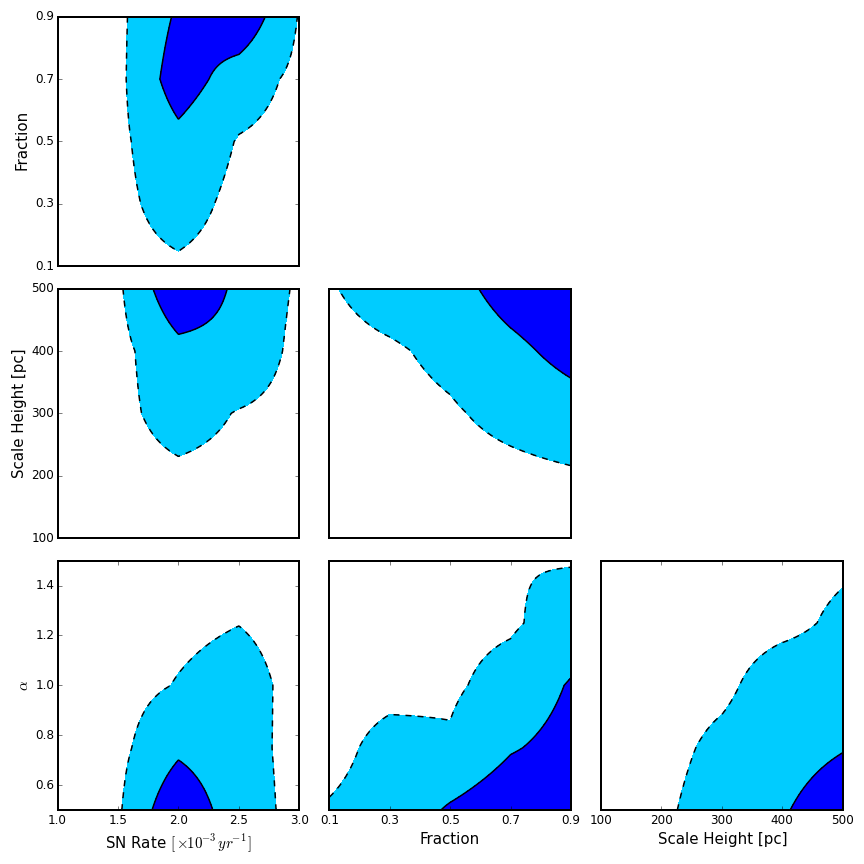
\includegraphics[width=15cm]{TrianglePlot_Diams.png}
\caption{}
\end{figure}
Diameter comparison sucks! I'll talk more about this.
\newpage
\section* {Density Comparison ($L_{cut} = 2 \times 10^{23}\ ergs/s/Hz$)}
\begin{figure}[h!]
%\vspace{5cm}
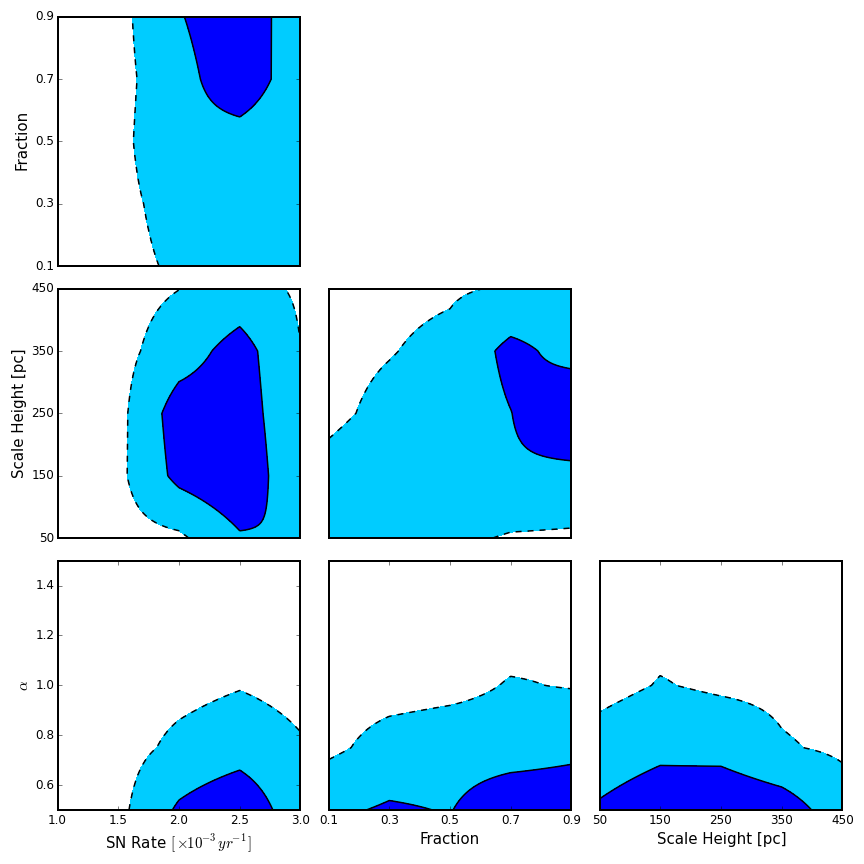
\includegraphics[width=15cm]{TrianglePlot_Dens.png}
\caption{}
\end{figure}
\newpage
\section* {Luminosity Comparison ($L_{cut} = 9 \times 10^{22}\ ergs/s/Hz$)}
\begin{figure}[h!]
%\vspace{-10cm}
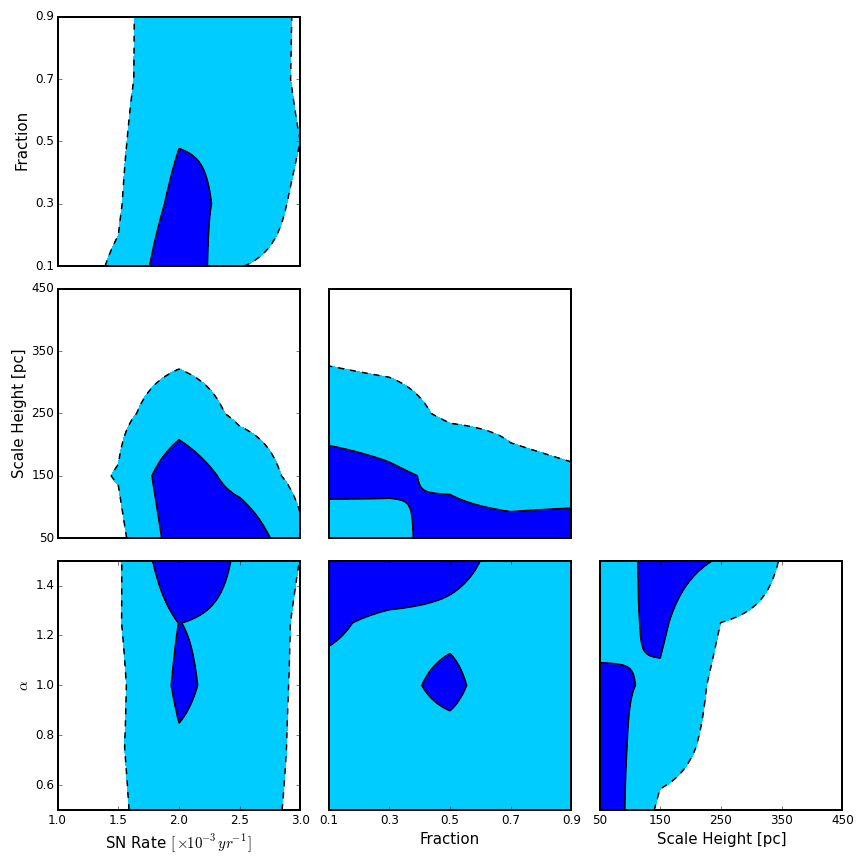
\includegraphics[width=15cm]{TrianglePlot_lums2.png}
\caption{Parameter Space constructed from comparing observed vs. model luminosity distribution for all Supernova brighter than $L_{cut}$. 65$\%$ region is shown in blue with solid border. 95$\%$ region is shown in cyan with dashed border.}
\end{figure}
\newpage
\section* {Diameter Comparison ($L_{cut} = 9 \times 10^{22}\ ergs/s/Hz$)}
\begin{figure}[h!]
%\vspace{-10cm}
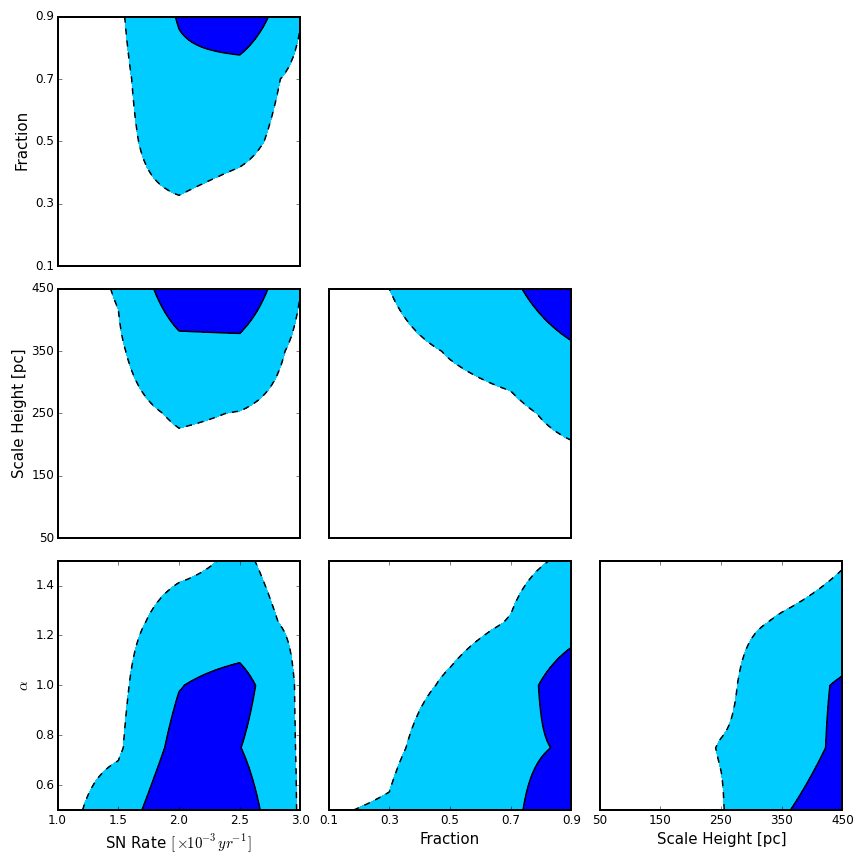
\includegraphics[width=15cm]{TrianglePlot_diams2.png}
\caption{}
\end{figure}
\newpage
\section* {Density Comparison ($L_{cut} = 9 \times 10^{22}\ ergs/s/Hz$)}
\begin{figure}[h!]
%\vspace{5cm}
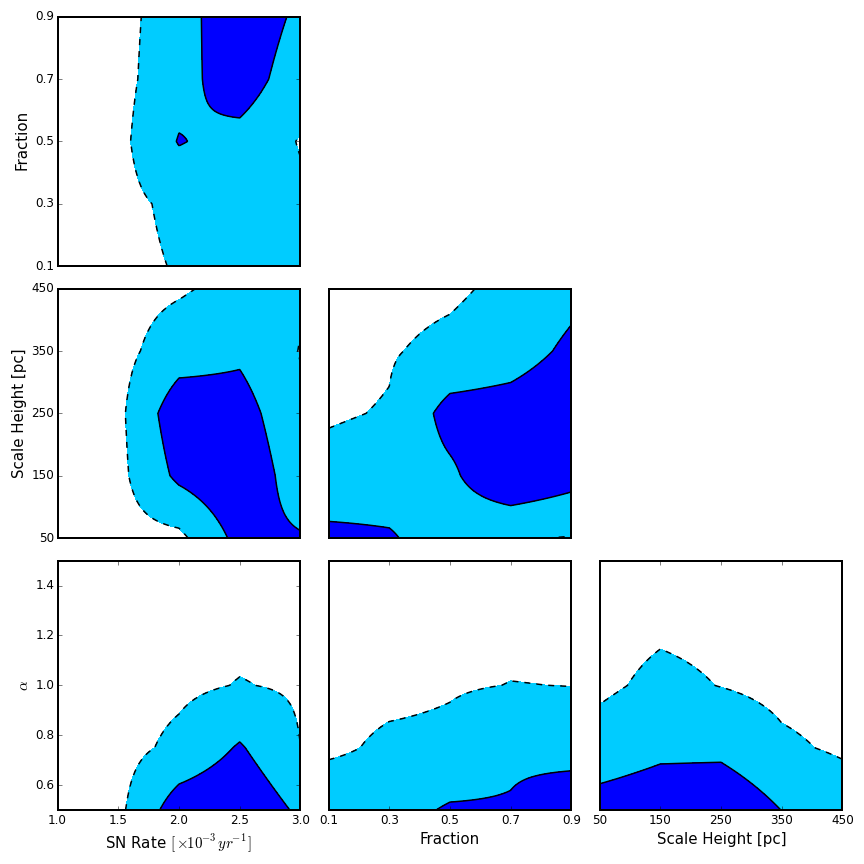
\includegraphics[width=15cm]{TrianglePlot_dens2.png}
\caption{}
\end{figure}

\end{document}
